\chapter{Manual Técnico y Despliegue}
\label{appendix:manual}

\section{Estructura del Proyecto}
El código fuente de la aplicación se organiza siguiendo el patrón de diseño de Flask \cite{flask}. A continuación se muestra la estructura de directorios principal y la función de cada módulo:

\begin{verbatim}
/tfg-web-ci-python
|-- .github/            # Flujos de CI/CD (GitHub Actions)
|-- app/
|   |-- data/           # Datos estáticos (JSON)
|   |-- static/         # CSS, JS e imágenes
|   |-- templates/      # Plantillas HTML (Jinja2)
|   |-- __init__.py     # Factoría de la aplicación
|   |-- career.py       # Lógica del "Modo Carrera"
|   `-- routes.py       # Controlador (Rutas)
|-- tests/              # Tests unitarios (pytest)
|-- requirements.txt    # Dependencias
`-- run.py              # Entry point
\end{verbatim}

\section{Instalación Local}
Para ejecutar el entorno de desarrollo se requieren Python 3.11+ \cite{python} y Git \cite{progit}.

\begin{enumerate}
    \item \textbf{Clonar el repositorio:}
    \begin{verbatim}
    git clone https://github.com/sanlaja/tfg-web-ci-python.git
    cd tfg-web-ci-python
    \end{verbatim}
    
    \item \textbf{Crear un entorno virtual e instalar dependencias:}
    \begin{verbatim}
    python -m venv .venv
    # En Windows:
    .venv\Scripts\activate
    # En Mac/Linux:
    source .venv/bin/activate
    
    pip install -r requirements.txt
    \end{verbatim}
    
    \item \textbf{Ejecutar la aplicación:}
    \begin{verbatim}
    python run.py
    \end{verbatim}
    El servidor estará accesible localmente en \texttt{http://localhost:5000}.
\end{enumerate}

\section{Despliegue en Render (Producción)}

El proyecto está configurado para desplegarse automáticamente en la plataforma en la nube \textbf{Render} \cite{render} mediante integración continua.

Para garantizar la estabilidad del servicio en el plan gratuito (limitado a 512 MB de RAM), ha sido necesario establecer la siguiente configuración de entorno en el servidor:

\begin{itemize}
    \item \texttt{PYTHON\_VERSION}: \texttt{3.11.0} (o superior) para asegurar compatibilidad.
    \item \texttt{WEB\_CONCURRENCY}: \texttt{1}. Esta variable es crítica para limitar a Gunicorn a un solo proceso \textit{worker}. Sin esta configuración, el servidor intenta instanciar múltiples procesos paralelos, agotando la memoria disponible al cargar librerías científicas como \texttt{pandas}, lo que provocaría los errores de memoria (\textit{OOM}) descritos en el capítulo de pruebas.
\end{itemize}

La versión de producción es accesible públicamente en:
\begin{center}
\texttt{https://tfg-web-ci-python.onrender.com}
\end{center}


\chapter{Manual de Usuario}
\label{appendix:manual_usuario}

Este manual guía cada pantalla del simulador con explicaciones detalladas, ejemplos numéricos y referencias directas al funcionamiento del sistema. El objetivo es que, incluso sin experiencia previa, cualquier usuario pueda entender qué significa cada campo, por qué importa y dónde aparece.

\section{Introducción Rápida}
El simulador tiene dos modos independientes:

\begin{itemize}
    \item \textbf{Modo Práctica:} Analizas un único \textit{ticker} con tus propios supuestos.
    \item \textbf{Modo Carrera:} Gestionas una sesión con varios turnos, eventos aleatorios y un ranking global.
\end{itemize}

Flujo recomendado para principiantes:
\begin{enumerate}
    \item Busca un \textit{ticker} con el pre-check de Yahoo Finance.
    \item Pruébalo en \textbf{Modo Práctica}.
    \item Crea una sesión de \textbf{Modo Carrera} con ese universo de activos.
    \item Respeta siempre las reglas clave: la suma de pesos no puede superar el 100\% ($\le 1.0$) y el máximo de activos es 10.
\end{enumerate}

\section{Conceptos Básicos Imprescindibles}
\begin{description}
    \item[Ticker] Símbolo bursátil en mayúsculas (ej. \texttt{AAPL}).
    \item[Benchmark] Índice de referencia para comparar tu cartera. Por defecto es el S\&P 500 (\texttt{\^{}GSPC}).
    \item[Cartera] Lista de activos con sus pesos asignados.
    \item[Turno] Intervalo de tiempo definido por una fecha de inicio y fin.
    \item[SOT (Start of Turn)] Capital y pesos en el instante previo a los eventos; sirve para medir variaciones.
    \item[DCA] Aportación automática (\textit{Dollar Cost Averaging}) que se suma al capital en cada turno.
\end{description}

\section{Modo Práctica Paso a Paso}
\begin{enumerate}
    \item \textbf{Formulario:} Completa ticker, importe (ej. 1.000 €), horizonte en años y fechas.
    \item \textbf{Validaciones:} El sistema exige importes positivos y fechas ordenadas.
    \item \textbf{DCA:} Elige entre inversión única o aportaciones periódicas.
    \item \textbf{Métricas:} Tras enviar, se calculan CAGR, \textit{drawdown} y PnL.
    \item \textbf{Historial:} Puedes guardar los resultados y exportar a CSV.
\end{enumerate}

\begin{figure}[h]
    \centering
    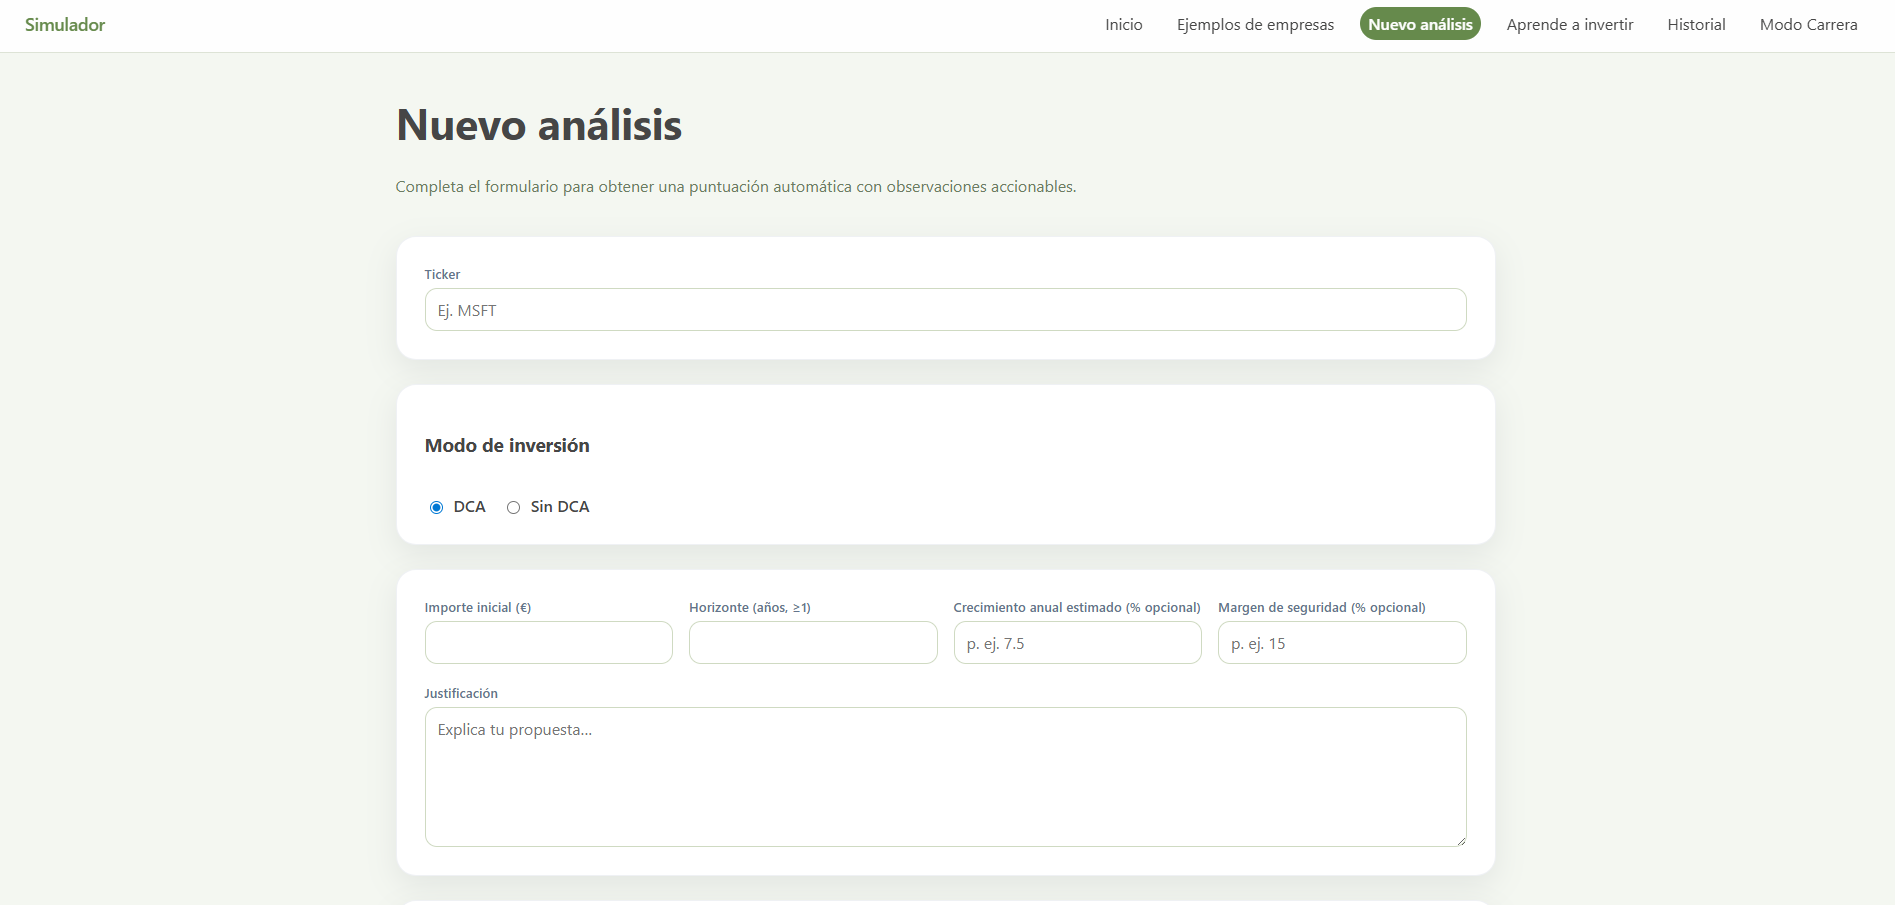
\includegraphics[width=0.8\textwidth]{figs/analisis_form.png}
    \caption{Pantalla del Modo Práctica.}
    \label{fig:modo_practica}
\end{figure}

\section{Modo Carrera Paso a Paso}
\begin{enumerate}
    \item \textbf{Crear sesión:} Define dificultad, capital inicial y universo de activos.
    \item \textbf{Asignar pesos:} El formulario valora hasta 10 activos. La suma debe ser $\le 1.0$.
    \item \textbf{Cerrar turno:} El sistema confirma que los datos son coherentes y avanza el tiempo.
    \item \textbf{Eventos:} Tras cerrar, aparece un resumen de eventos aleatorios (noticias, crisis).
    \item \textbf{Drift automático:} Los pesos del siguiente turno se ajustan automáticamente según la evolución del mercado.
    \item \textbf{Informe:} Genera un reporte final con métricas y posición en el ranking.
\end{enumerate}

\begin{figure}[h]
    \centering
    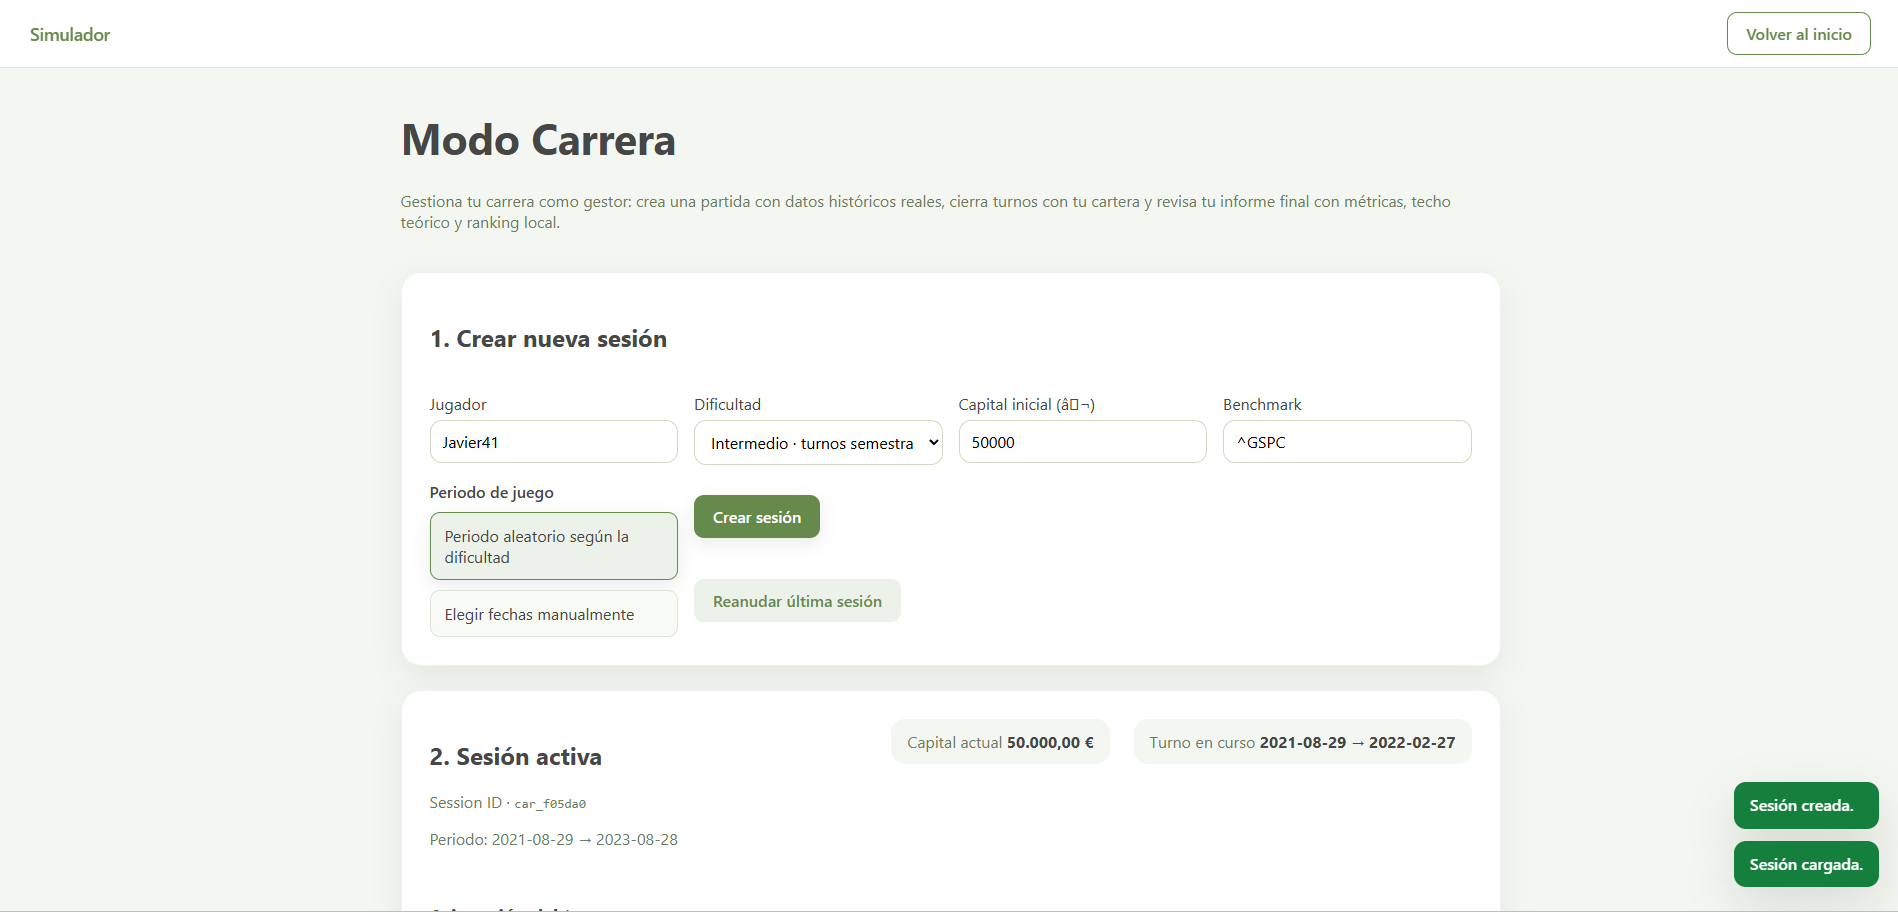
\includegraphics[width=0.9\textwidth]{figs/modo_carrera.png}
    \caption{Interfaz principal del Modo Carrera.}
    \label{fig:modo_carrera_ui}
\end{figure}

\section{Métricas y Tracking}
El informe genera dos series comparativas en Base 100 (Cartera vs Benchmark) y calcula:

\begin{itemize}
    \item \textbf{CAGR:} Crecimiento anual compuesto.
    \item \textbf{Max Drawdown:} Caída máxima desde el último pico.
    \item \textbf{Volatilidad Anual:} Desviación estándar del rendimiento.
    \item \textbf{Information Ratio:} Mide la consistencia del exceso de retorno sobre el benchmark.
\end{itemize}

\section{Glosario Completo}
\begin{description}
    \item[Ticker] Identificador oficial de una empresa. Ejemplo: \texttt{"MSFT"}.
    \item[Alloc] Asignación de pesos de la cartera. Ejemplo: \texttt{[{"ticker":"AAPL","weight":0.4}]}.
    \item[Efectivo (CASH)] Ticker especial para mantener liquidez sin invertir.
    \item[Snapshot] Registro completo del estado de un turno.
    \item[DCA] Estrategia de inversión constante para suavizar la entrada al mercado.
    \item[PnL (Abs/Pct)] Beneficio o pérdida en términos absolutos (€) o relativos (\%).
    \item[Base 100] Escala normalizada que comienza en 100 para comparar activos distintos.
    \item[Seed] Semilla aleatoria que permite replicar exactamente una sesión de simulación.
\end{description}

\section{Preguntas Frecuentes (FAQ)}
\textbf{¿Puedo dejar parte de la cartera en efectivo?} \\
Sí. Usa el ticker \texttt{CASH} o deja la suma de pesos por debajo de 1.0.

\textbf{¿Qué hago si un ticker no aparece?} \\
Revisa el buscador de Yahoo Finance. Si no tiene datos históricos suficientes, el sistema lo rechazará.

\textbf{¿Por qué cambian mis pesos automáticamente?} \\
Debido al "drift" de mercado: los activos que suben de precio ganan peso relativo en la cartera automáticamente.